\documentclass[a4paper,10pt,twocolumn,uplatex]{jsarticle}
\usepackage{style/nislab,style/resume}

%---------------------------------------------------------------------
% レジュメ種別・日付設定(要変更)
% \type{} 1:修士論文諮問会 2:卒業論文発表会 3:月例発表会 4:研究室合同発表会
%---------------------------------------------------------------------
\type{3}
\year{2022}
\month{10}
\date{8}

%---------------------------------------------------------------------
% ページ番号設定(要変更)
%---------------------------------------------------------------------
\setcounter{page}{1}

%---------------------------------------------------------------------
% 変更不要
%---------------------------------------------------------------------
\begin{document}

%---------------------------------------------------------------------
% タイトル作成部分(要変更)
% \maketitle{タイトル}{title}{名前}{name}
%---------------------------------------------------------------------
\maketitle{SDNを利用したQoS予測・予約によるV2X通信の信頼性向上}
{Improvement of V2X Communication Reliability\\by QoS Prediction \& Reservation Using SDN}
{国本 典晟}
{Tensei KUNIMOTO}

%---------------------------------------------------------------------
\section{はじめに}
自動運転やV2X通信について説明
基地局やアクセスポイントを通じることを説明
車両の集中により十分通信帯域が確保できないことを説明(参考文献)
提案手法へのつなぎ

%---------------------------------------------------------------------
\section{提案手法}
\subsection{SDNを利用したQoS予測}
SDNの説明
QoS予測の説明

\begin{figure}[t]
	\begin{centering}
    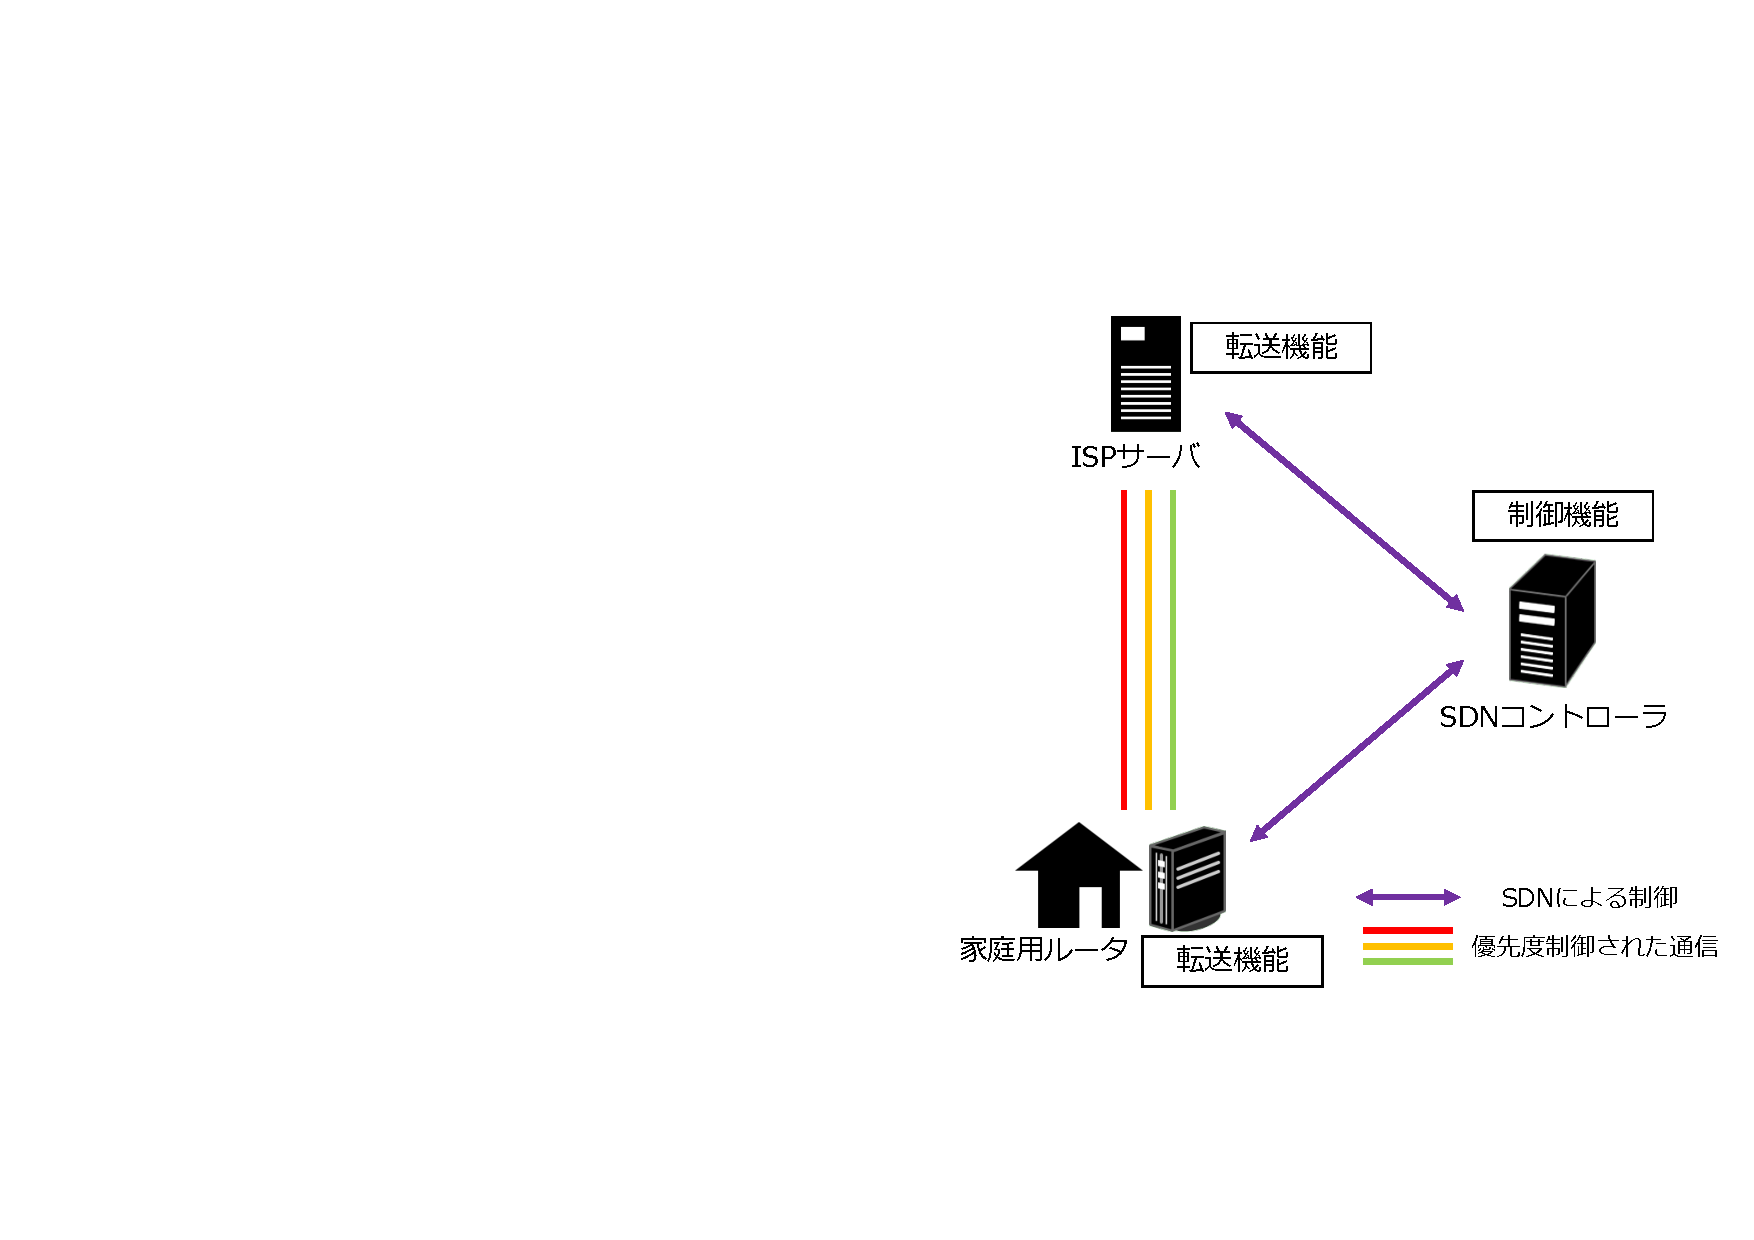
\includegraphics[width=0.7\linewidth]{img/proposal_resume.pdf}
    \caption{SDNを用いた通信制御}
    \label{fig:proposal}
    \end{centering}
\end{figure}

%---------------------------------------------------------------------
\subsection{QoS予測に基づくネットワーク制御}
\label{priority}
車両の走行経路
基地局(AP)とのやり取りも必要

%---------------------------------------------------------------------
\subsection{QoS予約}

%---------------------------------------------------------------------
\section{シミュレーションによる評価}
\subsection{シミュレーションモデル}
シミュレーションモデルを図付きで説明
シミュレーションモデルの条件を説明

%---------------------------------------------------------------------
\subsection{評価項目}
評価項目
比較対象

%---------------------------------------------------------------------
\section{まとめ}


%---------------------------------------------------------------------
% Bibliography(参考文献)
%---------------------------------------------------------------------
% thebibliography を利用する場合は以下を使用
\footnotesize{
  \begin{thebibliography}{99}
    \bibitem{ガイドライン} 総務省,帯域制御の運用基準に関するガイドライン(改定), 2019.
    \bibitem{AQRA} Guo-Cin Deng and Kuochen Wang, An Application-aware QoS Routing Algorithm for SDN-based IoT Networking, \textit{2018 IEEE Symposium on Computers and Communications (ISCC)}, pp. 186-191, 2018.
  \end{thebibliography}
}

% BibTex を利用する場合は以下を使用(初めての人には難しいかも)
% \bibliographystyle{junsrt}
% \bibliography{myref}

%---------------------------------------------------------------------
\end{document}
%---------------------------------------------------------------------
